\documentclass[11pt,a4paper]{article}

\usepackage[T1]{fontenc}
\usepackage[utf8]{inputenc}
\usepackage[french]{babel}
\usepackage{amsmath,amssymb}
\usepackage[margin=2.5cm]{geometry}
\usepackage{enumitem}
\usepackage{graphicx}

% Symboles d'indépendance
\newcommand{\indep}{\perp\!\!\!\perp}
\newcommand{\nindep}{\not\!\perp\!\!\!\perp}

% Mise en forme des conclusions
\newcommand{\conclusion}[1]{%
  \begin{center}\setlength{\fboxsep}{6pt}\fbox{#1}\end{center}}

\title{Question 4}

\begin{document}
\maketitle

\begin{center}
  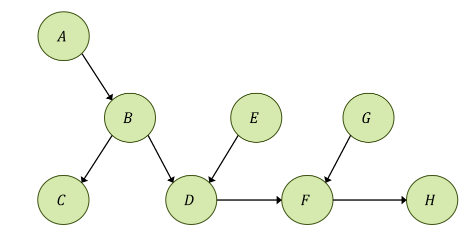
\includegraphics[width=0.9\textwidth]{q4.png}
\end{center}

\section*{a) Assertions d'indépendance}

\begin{enumerate}[label=(\roman*), leftmargin=*, itemsep=1.5em]

% ---------------------------------------------------------------- (i)
\item On considère le parcours $A \to B \to D \to F \leftarrow G$.
Ce parcours est actif étant donné $H$ car :
\begin{itemize}
  \item $A \to B \to D$ et $B \notin \{H\}$
  \item $B \to D \to F$ et $D \notin \{H\}$
  \item $D \to F \leftarrow G$ et $H$ est un descendant de $F$
\end{itemize}
Donc $(A,C)$ et $G$ ne sont pas d-séparés étant donné $H$, car il existe un parcours actif entre $A \in (A,C)$ et $G$ étant donné $H$.
\conclusion{Ainsi $(A,C) \indep G \mid H$ est \textbf{faux}.}

% --------------------------------------------------------------- (ii)
\item Le seul parcours reliant $E$ et $G$ est $E \to D \to F \leftarrow G$, qui passe par la v-structure $D \to F \leftarrow G$.
Or le n\oe ud $F$ et son descendant $H$ n'appartiennent pas à $\emptyset$.
Donc il n'existe pas de parcours actif entre $E$ et $G$ étant donné $\emptyset$ : ils sont d-séparés étant donné $\emptyset$.
\conclusion{Ainsi $E \indep G \mid \emptyset$ est \textbf{vrai}.}

% -------------------------------------------------------------- (iii)
\item On considère le parcours $A \to B \to D \leftarrow E$.
Ce parcours est actif étant donné $H$ car :
\begin{itemize}
  \item $A \to B \to D$ et $B \notin \{H\}$
  \item $B \to D \leftarrow E$ et $H$ est un descendant de $D$
\end{itemize}
Donc $A$ et $E$ ne sont pas d-séparés étant donné $H$, car il existe un parcours actif entre $A$ et $E$ étant donné $H$.
\conclusion{Ainsi $A \indep E \mid H$ est \textbf{faux}.}

% --------------------------------------------------------------- (iv)
\item On considère le parcours $A \to B \to D \leftarrow E$.
Ce parcours est actif étant donné $D$ car :
\begin{itemize}
  \item $A \to B \to D$ et $B \notin \{D\}$
  \item $B \to D \leftarrow E$ et $D \in \{D\}$
\end{itemize}
Donc $A$ et $(E,C)$ ne sont pas d-séparés étant donné $D$, car il existe un parcours actif entre $A$ et $E \in (E,C)$ étant donné $D$.
\conclusion{Ainsi $A \indep (E,C) \mid D$ est \textbf{faux}.}

% ---------------------------------------------------------------- (v)
\item Le seul parcours reliant $C$ et $E$ est $C \leftarrow B \to D \leftarrow E$, qui passe par la v-structure $B \to D \leftarrow E$.
Or le n\oe ud $D$ et tous ses descendants ($F$ et $H$) n'appartiennent pas à $\{A\}$.
Donc il n'existe pas de parcours actif entre $C$ et $E$ étant donné $A$ : $C$ et $E$ sont d-séparés étant donné $A$.
\conclusion{Ainsi $C \indep E \mid A$ est \textbf{vrai}.}

% --------------------------------------------------------------- (vi)
\item On considère le parcours $A \to B \to D \to F$.
Ce parcours est actif étant donné $\emptyset$ car :
\begin{itemize}
  \item $A \to B \to D$ et $B \notin \emptyset$
  \item $B \to D \to F$ et $D \notin \emptyset$
\end{itemize}
Donc $A$ et $F$ ne sont pas d-séparés étant donné $\emptyset$, car il existe un parcours actif entre $A$ et $F$ étant donné $\emptyset$.
\conclusion{Ainsi $A \indep F \mid \emptyset$ est \textbf{faux}.}

% -------------------------------------------------------------- (vii)
\item Tous les parcours reliant $C$ et $G$ passent par la structure $C \leftarrow B \to D$ et $B \in \{F,B\}$.
Donc il n'existe pas de parcours actif reliant $C$ et $G$ étant donné $\{F,B\}$ : $C$ et $G$ sont d-séparés étant donné $\{F,B\}$.
\conclusion{Ainsi $C \indep G \mid (F,B)$ est \textbf{vrai}.}

\end{enumerate}

\section*{b) SRB I-équivalentes}
 
L'affirmation est fausse car on trouve deux SRB I-équivalentes à celle donnée en a) et différentes de celle-ci.
On conserve les arêtes $B \to D \leftarrow E$, $D \to F \leftarrow G$ et $F \to H$ et on modifie seulement l'orientation de $A - B - C$ sans créer de nouvelle v-structure :
\begin{itemize}
  \item en changeant l'arête entre $A$ et $B$ pour avoir $A \leftarrow B$ (et $B \to C$ inchangée), on obtient un graphe différent, avec le même squelette et les mêmes immoralités ;
  \item en changeant l'arête entre $A$ et $B$ et celle entre $B$ et $C$ pour avoir $A \leftarrow B$ et $B \leftarrow C$, on obtient un autre graphe différent, toujours avec les mêmes immoralités et le même squelette.
\end{itemize}
\conclusion{Ainsi l'affirmation est \textbf{fausse}.}

\section*{c) Graphe moral}
 
\subsection*{(i)}
 
On souhaite montrer que si $X_A$ et $X_B$ sont séparés dans $\mathcal{H}_\mathcal{G}$ étant donné $\mathbf{Z}$, alors ils sont d-séparés dans $\mathcal{G}$ étant donné $\mathbf{Z}$. On montre la contraposée :
s'il existe un parcours actif entre $X_A$ et $X_B$ dans $\mathcal{G}$ étant donné $\mathbf{Z}$, alors il existe un chemin entre $X_A$ et $X_B$ dans $\mathcal{H}_\mathcal{G}$ qui ne passe par aucun n\oe ud de $\mathbf{Z}$.
 
Soit $X_A = V_0, V_1, \dots, V_k = X_B$ un parcours actif dans $\mathcal{G}$ étant donné $\mathbf{Z}$. Par définition d'un parcours actif, pour chaque triplet consécutif $(V_{i-1}, V_i, V_{i+1})$ du parcours :
\begin{itemize}
  \item si le triplet est de la forme $V_{i-1} \to V_i \to V_{i+1}$ ou $V_{i-1} \leftarrow V_i \leftarrow V_{i+1}$ ou $V_{i-1} \leftarrow V_i \to V_{i+1}$, alors $V_i \notin \mathbf{Z}$ ;
  \item si le triplet est une v-structure $V_{i-1} \to V_i \leftarrow V_{i+1}$, alors $V_i$ ou l'un de ses descendants appartient à $\mathbf{Z}$, ce qui peut poser problème pour la construction d'un chemin dans $\mathcal{H}_\mathcal{G}$.
\end{itemize}
 
\paragraph{On court-circuite chaque v-structure.}
Pour une v-structure $V_{i-1} \to V_i \leftarrow V_{i+1}$, les n\oe uds $V_{i-1}$ et $V_{i+1}$ sont deux parents de $V_i$. Par définition du graphe moral, $V_{i-1} - V_{i+1} \in \mathcal{L}'$. On peut donc remplacer $V_{i-1}, V_i, V_{i+1}$ par $V_{i-1}, V_{i+1}$ dans $\mathcal{H}_\mathcal{G}$, ce qui évite $V_i$.

\paragraph{Le chemin obtenu évite $\mathbf{Z}$.}
Après avoir court-circuité toutes les v-structures, il reste $X_A$, $X_B$ et les n\oe uds centraux des chaînes et des fourches du parcours initial, qui sont tous hors de $\mathbf{Z}$. Deux n\oe uds consécutifs sont reliés dans $\mathcal{H}_\mathcal{G}$ : soit ils étaient adjacents dans $\mathcal{G}$ (et l'arête devient non orientée dans $\mathcal{L}'$), soit ils étaient les deux parents d'un même n\oe ud central d'une v-structure (et l'arête vient de la moralisation). On obtient un chemin de $X_A$ à $X_B$ dans $\mathcal{H}_\mathcal{G}$ qui ne passe par aucun n\oe ud de $\mathbf{Z}$.

\conclusion{Ainsi, si $X_A$ et $X_B$ sont séparés dans $\mathcal{H}_\mathcal{G}$ étant donné $\mathbf{Z}$, alors ils sont d-séparés dans $\mathcal{G}$ étant donné $\mathbf{Z}$.}
 
\subsection*{(ii)}
 
La réciproque est \textbf{fausse}. On utilise un contre-exemple avec le graphe de a), en prenant $\mathbf{Z} = \emptyset$ :
\begin{itemize}
  \item $B$ et $E$ sont d-séparés dans $\mathcal{G}$ étant donné $\emptyset$ : le seul parcours entre eux est $B \to D \leftarrow E$, et le n\oe ud $D$ au centre de la v-structure (ainsi que ses descendants $F$ et $H$) n'appartient pas à $\emptyset$, le parcours n'est donc pas actif.
  \item mais $B$ et $E$ sont les deux parents de $D$, donc l'arête $B - E$ appartient à $\mathcal{L}'$. Ils sont adjacents dans $\mathcal{H}_\mathcal{G}$ et ne sont donc pas séparés étant donné $\emptyset$.
\end{itemize}

\begin{center}
  \fbox{\parbox{0.9\textwidth}{\centering Ainsi, si $X_A$ et $X_B$ sont d-séparés dans $\mathcal{G}$ étant donné $\mathbf{Z}$, alors ils ne sont pas forcément séparés dans $\mathcal{H}_\mathcal{G}$ étant donné $\mathbf{Z}$.}}
\end{center}

\end{document}